%%%% CS553 Cryptography Term Paper TEMPLATE %%%%

%%%% 1. DOCUMENTCLASS %%%%
\documentclass[preprint]{transcrypto}
%%%% NOTES:
% - Change "submission" to "final" for final version
% - Add "spthm" for LNCS-like theorems


%%%% 2. PACKAGES %%%%
\usepackage{lipsum} % Example package -- can be removed
\usepackage{tabto}
\usepackage{float}
\restylefloat{table}
\usepackage{multirow}


%%%% 3. AUTHOR, INSTITUTE %%%%
\author{Walkie\_Talkie}
\institute{
  Ajay Tarole, \email{ajayt@iitbhilai.ac.in}
  \and
  Ashish Kumar Suraj, \email{ashishs@iitbhilai.ac.in}
  \and
  Vikash Vitthore, \email{vikashv@iitbhilai.ac.in}
}
%%%% NOTES:
% - We need a city name for indexation purpose, even if it is redundant
%   (eg: University of Atlantis, Atlantis, Atlantis)
% - \inst{} can be omitted if there is a single institute,
%   or exactly one institute per author


%%%% 4. TITLE %%%%
\title[SKINNY CIPHER]{Term Paper on SKINNY CIPHER}
%%%% NOTES:
% - If the title is too long, or includes special macro, please
%   provide a "running title" as optional argument: \title[Short]{Long}
% - You can provide an optional subtitle with \subtitle.

\begin{document}

\maketitle


%%%% 5. KEYWORDS %%%%
\keywords{lightweight encryption \and tweakable block cipher}


%%%% 6. ABSTRACT %%%%
\begin{abstract}
	SKINNY is a new tweakable block cipher(family of lightweight tweakable block ciphers), The goal is to have draw contrast on different aspects of cipher. Doing analysis of its security with regards to much stronger ciphers. SKINNY has flexible block/key/tweak sizes protection and has the smallest total number of AND/OR/XOR gates used for encryption process. In this paper, we present zero-correlation linear approximations and the related-tweakey impossible differential characteristics for SKINNY. Regarding performances, it outperforms all known ciphers for ASIC round-based implementations, while still reaching an extremely small area for serial implementations and a very good efficiency for software and micro-controllers implementations.
\end{abstract}


%%%% 7. PAPER CONTENT %%%%
\section{Introduction}

$\quad\quad$ Due to the increasing importance of pervasive computing, lightweight cryptography is
currently a very active research domain in the symmetric-key cryptography community.
In particular, we have recently seen the apparition of many (some might say too many)
lightweight block ciphers, hash functions and stream ciphers. the efficiency on different hardware technologies (ASIC, FPGA) needs to be taken into account, and even micro-controllers become a scenario of importance. Finally, as remarked in software im- plementations should not be completely ignored for these  primitives, as in many applications the tiny devices will communicate with servers handling thousands or millions of them. Thus, even so research started by focusing on chip area only, lightweight cryptography is indeed an inherent multidimensional problem.
\\ 
\tab $\quad\quad$ Investigating the recent proposals in more detail, a major distinction is eye-catching
and one can roughly split the proposals in two classes. The first class of ciphers uses very
strong, but less efficient components (like the Sbox used in PRESENT  or LED , or
the MDS diffusion matrix in LED or PICCOLO). The second class of designs uses very
efficient, but rather weak components (like the very small KATAN or SIMON  round function). From a security viewpoint, the analysis of the members of the first class can be conducted much easily and it is usually possible to derive strong arguments for their security. However, while the second class strategy usually gives very competitive performance figures, it is much harder with state-of-the-art analysis techniques to obtain security guarantees even with regards to basic linear or differential cryptanalysis.
\\
\tab $\quad\quad$ The  publication of the SIMON and SPECK family of block ciphers by the NSA. Those ciphers brought a huge leap in terms of performances. As of today, these two primitives have an important efficiency advantage against all its competitors, in almost all implementation scenarios and platforms. However, even though SIMON or SPECK are quite elegant and seemingly well-crafted designs, these efficiency improvements came at an essential price. 
\\
\tab $\quad\quad$ Lightweight Tweakable Block Ciphers and Side-Channel Protected Implemen-
tations. We note that tiny devices are more prone to be deployed into insecure environ-
ments and thus side-channel protected implementations of lightweight encryption primitives
is a very important aspect that should be taken care of. One might even argue that instead
of comparing performances of unprotected implementations of these lightweight primitives,
one should instead compare protected variants (this is the recent trend followed by ciphers
like ZORRO or PICARO  and has actually already been taken into account long before by the cipher NOEKEON). One extra protection against side-channel attacks can be the use of leakage resilient designs and notably through an extra tweak input of the cipher. Such tweakable block ciphers are rather rare, the only such candidate being Joltik-BC or the internal cipher from SCREAM . Coming up with a tweakable block cipher is indeed not an easy task as one must be extremely careful how to include this extra input that
can be fully controlled by the attacker.
\\
\tab $\quad\quad$ Low-Latency Implementations for Memory Encryption. One very interesting field
in the area of lightweight cryptography is memory encryption. Memory encryption has been used in the literature to protect the memory used by a process domain against several types of attackers, including attackers capable of monitoring and even manipulating bus trans-
actions. Examples of commercial uses do not abound, but there are at least two: IBM’s
SecureBlue++  and Intel’s SGX whose encryption and integrity mechanisms have been
presented by Gueron at RWC 2016. 2 No documentation seems to be publicly available
regarding the encryption used in IBM’s solution, while Intel’s encryption method requires
additional data to be stored with each cache line. It is optimal in the context of encryption
with memory overhead, but if the use case does not allow memory overhead then an entirely
different approach is necessary.
\\
\tab $\quad\quad$ SKINNY is an SPN cipher that uses a compact Sbox. Some versions of SKINNY have a very large key size compared to its block size and this theoretically renders the bounds search space huge. With regard to performance, SKINNY reaches very small area with serial ASIC implementations, yet it is actually the very first block cipher that leads to better performances
than SIMON

\section{Specifications}

\paragraph{Notations.}
$\\$
This Cipher have 64-bit and 128-bit block versions. In both n=64 and n=128 versions, internal state can be viewed as 4*4 square array of cells. Each cell called a nibble or a byte. It has 3 main tweakey size versions: for a block size n, their are tweakey sizes available with t=n, t=2n and t=3n and z=t/n the tweakey size to block size ratio.
\paragraph{Initialization.}
$\\$
SKINNY receives a plaintext as usual done by any of the ciphers, it receives in the format of $m=m_0||m_1||\cdot\cdot\cdot||m_{14}||m_{15}$, where $m_i$ are s-bit cells. The initialization of the cipher's internal state is performed by simply setting $IS_i=m_i$ for 0 $\leq i \leq$ 15:
\begin{center}
	$IS=$
$\begin{bmatrix}
	m_0 & m_1 & m_2 & m_3\\
	m_4 & m_5 & m_6 & m_7\\
	m_8 & m_9 & m_{10} & m_{11}\\
	m_{12} & m_{13} & m_{14} & m_{15}
\end{bmatrix}$
\\ \end{center}
\tab This is the initial value of the cipher, the tate is loaded row-wise rather than in the column-wise fashion we have to expect from the AES.\\

\begin{table}[htb]
	\begin{center}
		\begin{tabular}{cccc}
		\hline
		\multicolumn{1}{l}{} & \multicolumn{3}{c}{Tweakey size t} \\ \cline{2-4} 
		Block size n         & n          & 2n        & 3n        \\ \hline
		64                   & 32 rounds  & 36 rounds & 40 rounds \\ \hline
		128                  & 40 rounds  & 48 rounds & 56 rounds \\ \hline
	\end{tabular}
	\end{center}

\caption{Number of rounds for SKINNY, with n-th bit internal state and t-bit tweakey state.}
\end{table}

\begin{figure}
\paragraph{Round function}
$\\$
One encryption round of SKINNY is composed of five operations in the following order: \textbf{SubCells, AddConstants(AC), AddRoundTweakey(ART), ShiftRows(SR)} and \textbf{MixColumns(MC)}

	\begin{center}
	\caption{It applies five different transformations: SC, AC, ART, SR, MC}
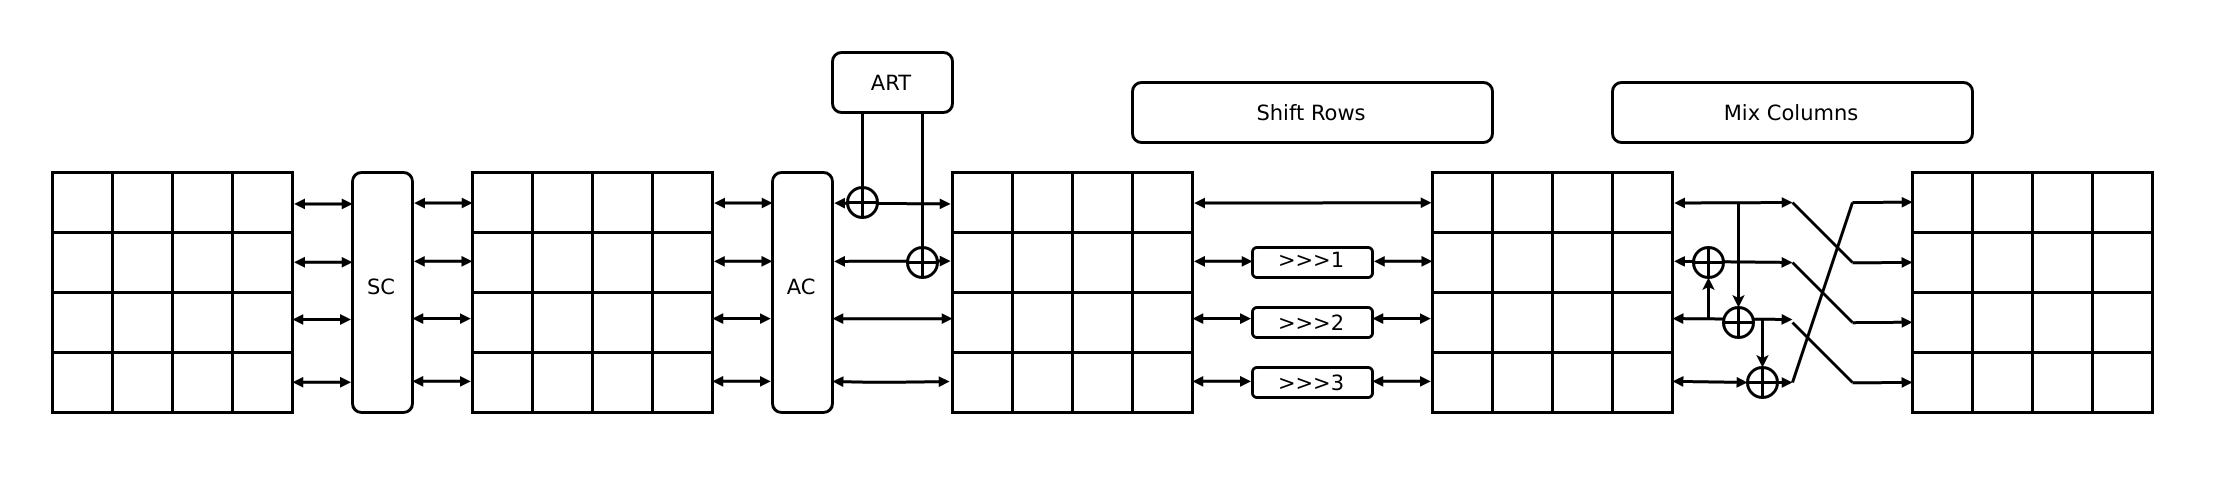
\includegraphics[width=10cm]{fig1.png}
	\end{center}
\end{figure}

\paragraph{1.SubCells}A s-bit Sbox is applied to every cell of the cipher internal state. let say for s = 4, SKINNY uses a Sbox $S_4$ very close to the Sbox of \textmd{PICCOLO}. $S_4$ can also be described with four NOR and four XOR operations.

\begin{center}
	($x_3,x_2,x_1,x_0$)$\rightarrow$($x_3,x_2,x_1,x_0\oplus(\overline{x_3\vee x_2}$)),\\
\end{center}
This process is repeated four times, except for the last iteration where the bit rotation is ommited.
\paragraph{2.AddConstants}The round constants whatever they are are combined with the state, respecting array positioning, using bitwise exclusive-or.
\begin{figure}[H]
	\paragraph{3.AddRoundTweakey}The first and second rows of all tweakey arrays are extracted and bitwise exclusive-ored to the cipher internal state, respecting the array positioning.
\begin{center}
	\caption{Each tweakey word $TK1,\ \ TK2\ \ and\ \ TK3$(if any) follows a similar transformation update, except that no LFSR is applied to TK1.}
	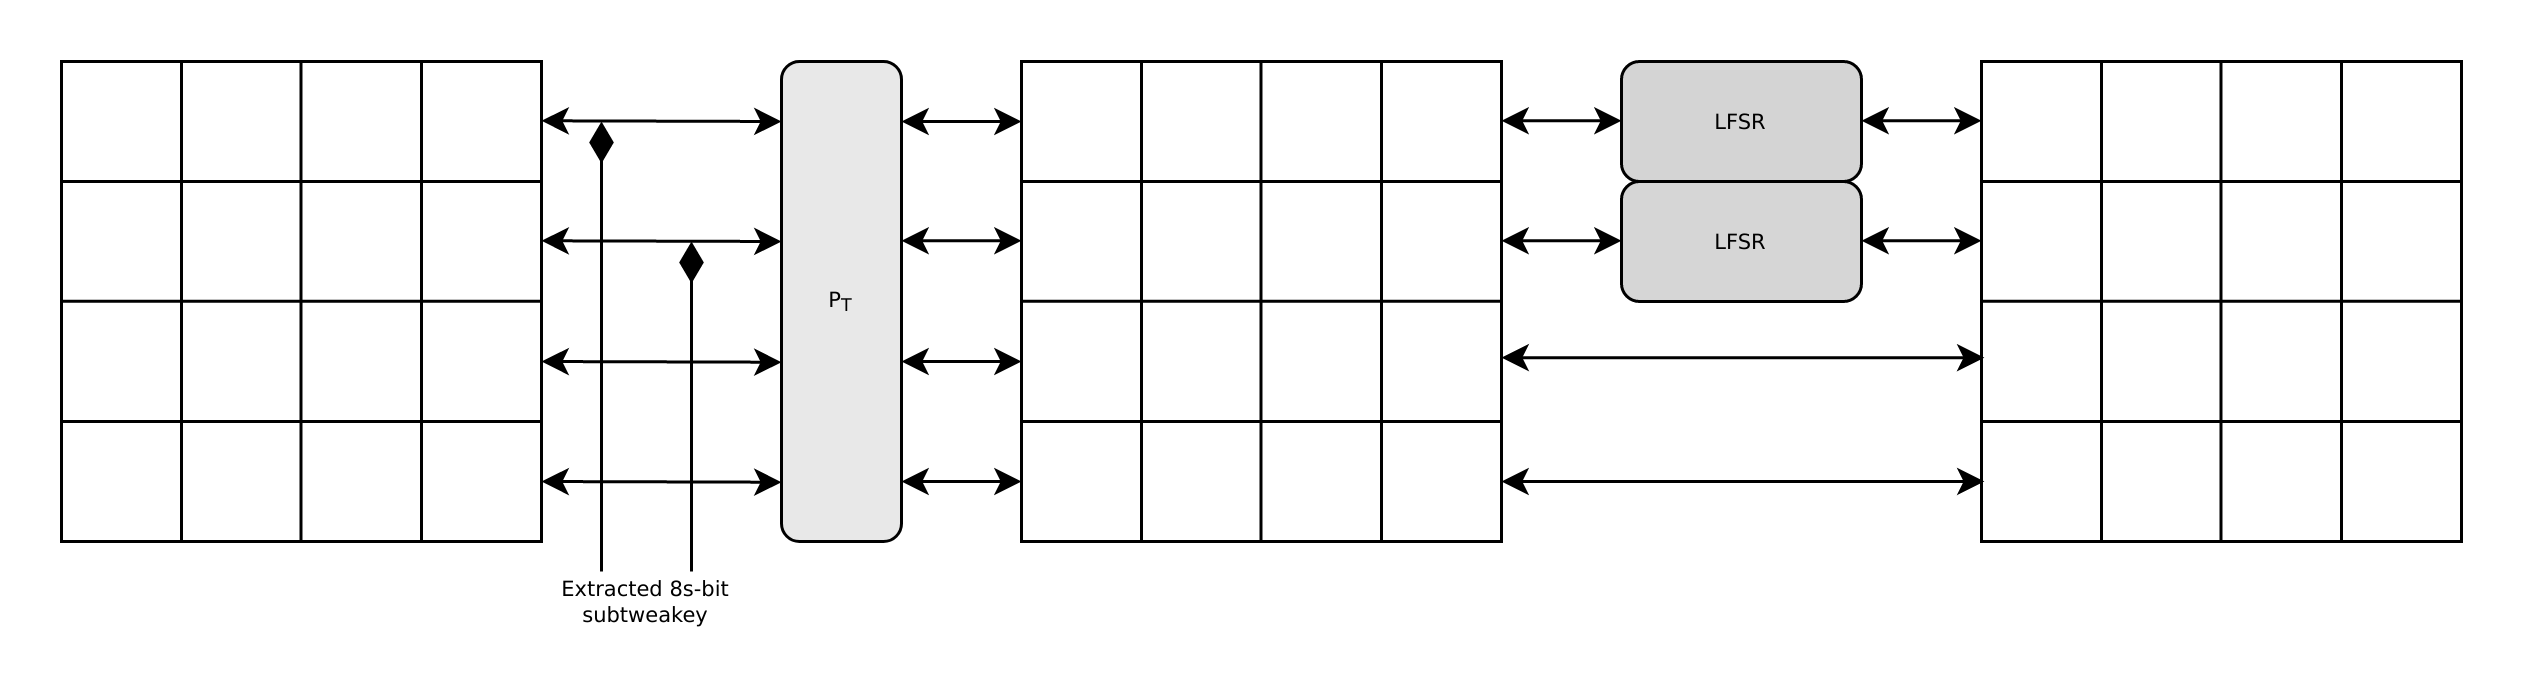
\includegraphics[width=10cm]{fig2.png}
\end{center}
\end{figure}
\paragraph{4.ShiftRows}In this layer the rows of the cipher state cell array are rotated, but they are to the right. The second, third and fourth cell rows are rotated by 1,2 and 3 positions to the right, respectively.
\paragraph{5.MixColumns}In this section, each column of the cipher internal state array is multiplied by a matrix M. (SubCells and MixColumns are based on a generalized Feistel structure, so their respective inverse is straightforward to deduce and can be implemented with the exact same number of operations.

\section{Rationale of SKINNY}
\tab Several design choices of SKINNY have been borrowed from existing ciphers, When designing SKINNY, one of our main criteria was to only add components
which are vital for the security of the primitive, removing any unnecessary operation
(hence the name of our proposal).
\\
\tab$\quad$ We note that one could have chosen a slightly smaller Sbox or a slightly sparser diffusion layer, but our preliminary implementations showed that these options represent worse tradeoff overall. For example, one could imagine a very simple cipher iterating thousands of rounds composed of only a single non-linear boolean operation, an XOR and some bit wiring. However, such a cipher will lead to terrible performance regarding throughput, latency or energy consumption.
\subsection{Comparing Differential Bounds}
\tab First, we emphasize that most of the bounds we obtained for SKINNY are not tight, and we can hope for even higher minimal numbers of active Sboxes. This is not the case of LED or PRESENT for which the bounds are tight.\\
Comparison between AES-128 and SIMON/SKINNY
	\begin{table}[htb]
\begin{center}
		\begin{tabular}{ccc}
			\hline
			Cipher                                                   & Single Key   & Related Key    \\ \hline
			SKINNY-64-128                                            & 8/36 = 0.22  & 15/36 = 0.42   \\
			SIMON-64-128                                             & 19/44 = 0.43 & no bound known \\ \hline
			SKINNY-128-128                                           & 15/40 = 0.37 & 19/40 = 0.47   \\
			\begin{tabular}[c]{@{}c@{}}SIMON-\\ 128-128\end{tabular} & 41/68 = 0.60 & no bound known \\
			AES-128                                                  & 4/10 = 0.40  & 6/10 = 0.60    \\ \hline
		\end{tabular}
	\end{center}
\caption{Comparision between AES-128 and SIMON/SKINNY versions for the proportion of total number of rounds needed to provide a sufficiently good differential characteristic.}.
\end{table}
\tab$\quad$ Finally, in terms of diffusion, all versions of SKINNY achieve full diffusion after only 6 rounds (forwards or backwards), while SIMON versions with 64-bit block size requires 9 rounds, and even 13 rounds for SIMON versions with 128-bit block size [27] (AES-128 reaches full diffusion after 2 of its 10 rounds). Again, the diffusion comparison according to the total number of rounds is at SKINNY’s advantage

\subsection{Comparing Theoretical Performance}
\tab One can see from the Table 3 that SIMON and SKINNY compare very favorably to
other candidates, both in terms of number of operations and theoretical area grade for
round-based implementations. This seems to confirm that when it comes to lightweight
block ciphers, SIMON is probably the strongest competitor as of today. Besides, SKINNY
has the best theoretical profile among all the candidates presented here, even better than
SIMON for area. For speed efficiency, SKINNY outperforms SIMON when the key schedule is
taken in account. This scenario is arguably the most important in practice. it is likely that lightweight devices will cipher very small messages and thus the
back-end servers communicating with millions of devices will probably have to recompute
the key schedule for every small message received.
\small{
\begin{table}[hbt]
	\tiny
	\centering
	\begin{tabular}{p{0.1\linewidth}p{0.11\linewidth}p{0.1\linewidth}p{0.09\linewidth}p{0.07\linewidth}p{0.08\linewidth}p{0.08\linewidth}p{0.12\linewidth}}
		\hline
		\multirow{2}{*}{Cipher} &
		\multirow{2}{*}{nb. of rds} &
		\multicolumn{3}{c}{gate cost (per bit per round)} &
		\multirow{2}{*}{nb. of op.} &
		\multirow{2}{*}{nb. of op.} &
		\multirow{2}{*}{\begin{tabular}[c]{@{}c@{}}round-based \\ impl. area\end{tabular}} \\ \cline{3-5}
		&
		&
		int. cipher &
		key sch. &
		total &
		&
		&
		\\ \hline
		\begin{tabular}[c]{@{}c@{}}SKINNY\\ -64-128\end{tabular} &
		36 &
		\begin{tabular}[c]{@{}c@{}}1N\\ 2.25 X\end{tabular} &
		0.625 X &
		\begin{tabular}[c]{@{}c@{}}1N\\ 2.875 X\end{tabular} &
		\begin{tabular}[c]{@{}c@{}}3.25 × 36\\ = 117\end{tabular} &
		\begin{tabular}[c]{@{}c@{}}3.875 × 36\\ = 139.5\end{tabular} &
		\begin{tabular}[c]{@{}c@{}}1 + 2.67 × 2.875\\ = 8.68\end{tabular} \\ \hline
		\begin{tabular}[c]{@{}c@{}}SIMON\\ -64/128\end{tabular} &
		44 &
		\begin{tabular}[c]{@{}c@{}}0.5 A\\ 1.5 X\end{tabular} &
		1.5 X &
		\begin{tabular}[c]{@{}c@{}}0.5 A\\ 3.0 X\end{tabular} &
		\begin{tabular}[c]{@{}c@{}}2 × 44\\ = 88\end{tabular} &
		\begin{tabular}[c]{@{}c@{}}3.5 × 44\\ = 154\end{tabular} &
		\begin{tabular}[c]{@{}c@{}}0.67 + 2.67 × 3\\ = 8.68\end{tabular} \\ \hline
		\begin{tabular}[c]{@{}c@{}}PRESENT\\ -128\end{tabular} &
		31 &
		\begin{tabular}[c]{@{}c@{}}1A\\ 3.75 X\end{tabular} &
		\begin{tabular}[c]{@{}c@{}}0.125 A\\ 0.344 X\end{tabular} &
		\begin{tabular}[c]{@{}c@{}}1.125 A\\ 4.094 X\end{tabular} &
		\begin{tabular}[c]{@{}c@{}}4.75 × 31\\ = 147.2\end{tabular} &
		\begin{tabular}[c]{@{}c@{}}5.22 × 31\\ = 161.8\end{tabular} &
		\begin{tabular}[c]{@{}c@{}}1.5 + 2.67 × 4.094\\ = 12.43\end{tabular} \\ \hline
		\begin{tabular}[c]{@{}c@{}}PICCOLO\\ -128\end{tabular} &
		31 &
		\begin{tabular}[c]{@{}c@{}}1N\\ 4.25 X\end{tabular} &
		&
		\begin{tabular}[c]{@{}c@{}}1N\\ 4.25 X\end{tabular} &
		\begin{tabular}[c]{@{}c@{}}5.25 × 31\\ = 162.75\end{tabular} &
		\begin{tabular}[c]{@{}c@{}}5.25 × 31\\ = 162.75\end{tabular} &
		\begin{tabular}[c]{@{}c@{}}1 + 2.67 × 4.25\\ = 12.35\end{tabular} \\ \hline
		\begin{tabular}[c]{@{}c@{}}KATAN\\ -64-80\end{tabular} &
		254 &
		\begin{tabular}[c]{@{}c@{}}0.047 N\\ 0.094 X\end{tabular} &
		3X &
		\begin{tabular}[c]{@{}c@{}}0.047 N\\ 3.094 X\end{tabular} &
		\begin{tabular}[c]{@{}c@{}}0.141 × 254\\ = 35.81\end{tabular} &
		\begin{tabular}[c]{@{}c@{}}3.141 × 254\\ = 797.8\end{tabular} &
		\begin{tabular}[c]{@{}c@{}}0.19+2.67×3.094\\ = 8.45\end{tabular} \\ \hline
		\begin{tabular}[c]{@{}c@{}}SKINNY\\ -128-128\end{tabular} &
		40 &
		\begin{tabular}[c]{@{}c@{}}1N\\ 2.25 X\end{tabular} &
		&
		\begin{tabular}[c]{@{}c@{}}1N\\ 2.25 X\end{tabular} &
		\begin{tabular}[c]{@{}c@{}}3.25 × 40\\ = 130\end{tabular} &
		\begin{tabular}[c]{@{}c@{}}3.25 × 40\\ = 130\end{tabular} &
		\begin{tabular}[c]{@{}c@{}}1 + 2.67 × 2.25\\ = 7.01\end{tabular} \\ \hline
		\begin{tabular}[c]{@{}c@{}}SIMON\\ -128/128\end{tabular} &
		68 &
		\begin{tabular}[c]{@{}c@{}}0.5 A\\ 1.5 X\end{tabular} &
		1X &
		\begin{tabular}[c]{@{}c@{}}0.5 A\\ 2.5 X\end{tabular} &
		\begin{tabular}[c]{@{}c@{}}2 × 68\\ = 136\end{tabular} &
		\begin{tabular}[c]{@{}c@{}}3 × 68\\ = 204\end{tabular} &
		\begin{tabular}[c]{@{}c@{}}0.67 + 2.67 × 2.5\\ = 7.34\end{tabular} \\ \hline
		\begin{tabular}[c]{@{}c@{}}NOEKEON\\ -128\end{tabular} &
		16 &
		\begin{tabular}[c]{@{}c@{}}0.5(A + N)\\ 5.25 X\end{tabular} &
		\begin{tabular}[c]{@{}c@{}}0.5(A + N)\\ 5.25 X\end{tabular} &
		\begin{tabular}[c]{@{}c@{}}1(A + N)\\ 10.5 X\end{tabular} &
		\begin{tabular}[c]{@{}c@{}}6.25 × 16\\ = 100\end{tabular} &
		\begin{tabular}[c]{@{}c@{}}12.5 × 16\\ = 200\end{tabular} &
		\begin{tabular}[c]{@{}c@{}}2.33 + 2.67 × 10.5\\ = 30.36\end{tabular} \\ \hline
		\begin{tabular}[c]{@{}c@{}}AES\\ -128\end{tabular} &
		10 &
		\begin{tabular}[c]{@{}c@{}}4.25 A\\ 16 X\end{tabular} &
		\begin{tabular}[c]{@{}c@{}}1.06 A\\ 3.5 X\end{tabular} &
		\begin{tabular}[c]{@{}c@{}}5.31 A\\ 19.5 X\end{tabular} &
		\begin{tabular}[c]{@{}c@{}}20.25 × 10\\ = 202.5\end{tabular} &
		\begin{tabular}[c]{@{}c@{}}24.81 × 10\\ = 248.1\end{tabular} &
		\begin{tabular}[c]{@{}c@{}}7.06 + 2.67 × 19.5\\ = 59.12\end{tabular} \\ \hline
		\begin{tabular}[c]{@{}c@{}}SKINNY\\ -128-256\end{tabular} &
		48 &
		\begin{tabular}[c]{@{}c@{}}1N\\ 2.25 X\end{tabular} &
		0.56 X &
		\begin{tabular}[c]{@{}c@{}}1N\\ 2.81 X\end{tabular} &
		\begin{tabular}[c]{@{}c@{}}3.25 × 48\\ = 156\end{tabular} &
		\begin{tabular}[c]{@{}c@{}}3.81 × 48\\ = 183\end{tabular} &
		\begin{tabular}[c]{@{}c@{}}1 + 2.67 × 2.81\\ = 8.5\end{tabular} \\ \hline
		\begin{tabular}[c]{@{}c@{}}SIMON\\ -128/256\end{tabular} &
		72 &
		\begin{tabular}[c]{@{}c@{}}0.5 A\\ 1.5 X\end{tabular} &
		1.5 X &
		\begin{tabular}[c]{@{}c@{}}0.5 A\\ 3.0 X\end{tabular} &
		\begin{tabular}[c]{@{}c@{}}2 × 72\\ = 144\end{tabular} &
		\begin{tabular}[c]{@{}c@{}}3.5 × 72\\ = 252\end{tabular} &
		\begin{tabular}[c]{@{}c@{}}0.67 + 2.67 × 3\\ = 8.68\end{tabular} \\ \hline
		\begin{tabular}[c]{@{}c@{}}AES\\ -256\end{tabular} &
		14 &
		\begin{tabular}[c]{@{}c@{}}4.25 A\\ 16 X\end{tabular} &
		\begin{tabular}[c]{@{}c@{}}2.12 A\\ 7X\end{tabular} &
		\begin{tabular}[c]{@{}c@{}}6.37 A\\ 23 X\end{tabular} &
		\begin{tabular}[c]{@{}c@{}}20.25 × 14\\ = 283.5\end{tabular} &
		\begin{tabular}[c]{@{}c@{}}29.37 × 14\\ = 411.2\end{tabular} &
		\begin{tabular}[c]{@{}c@{}}8.47 + 2.67 × 23\\ = 69.88\end{tabular} \\ \hline
	\end{tabular}
\caption{Total number of operations and theoretical performance of SKINNY and various lightweight block ciphers. N denotes NOR gate, A denotes a AND gate, X denotes a XOR gate.}
\end{table}

\section{Security Analysis}
\tab In this section, we provide an in-depth analysis of the security of the SKINNY family of block
ciphers. These models are based on related-key models.
\subsection{Integral attack}
\tab In this attack, we prepare a set of plaintext, so that particular cells can contain all the value in
the set, and other cells are fixed to a constant, after several round of encryption, we see the
changes of this encryption. For this we consider four properties All, Balanced, constant, unknown.
Definition of these for all following.\\ \\
\textbf{All} same number appear in the all cell.\\
\textbf{Balance} The sum of all values in the multiset is 0.\\
\textbf{Constant} The cell value is fixed through the multiset.\\
\textbf{Unknown}No particular property exists\\

\begin{figure}[H]
	\centering
			\caption{11-round impossible differential characteristic. SR and MC stand for ShiftRows and MixColumns, respectively. SubCells, AddColumns and AddTweakey are omitted since they are not related to the impossible differential characteristic.}
		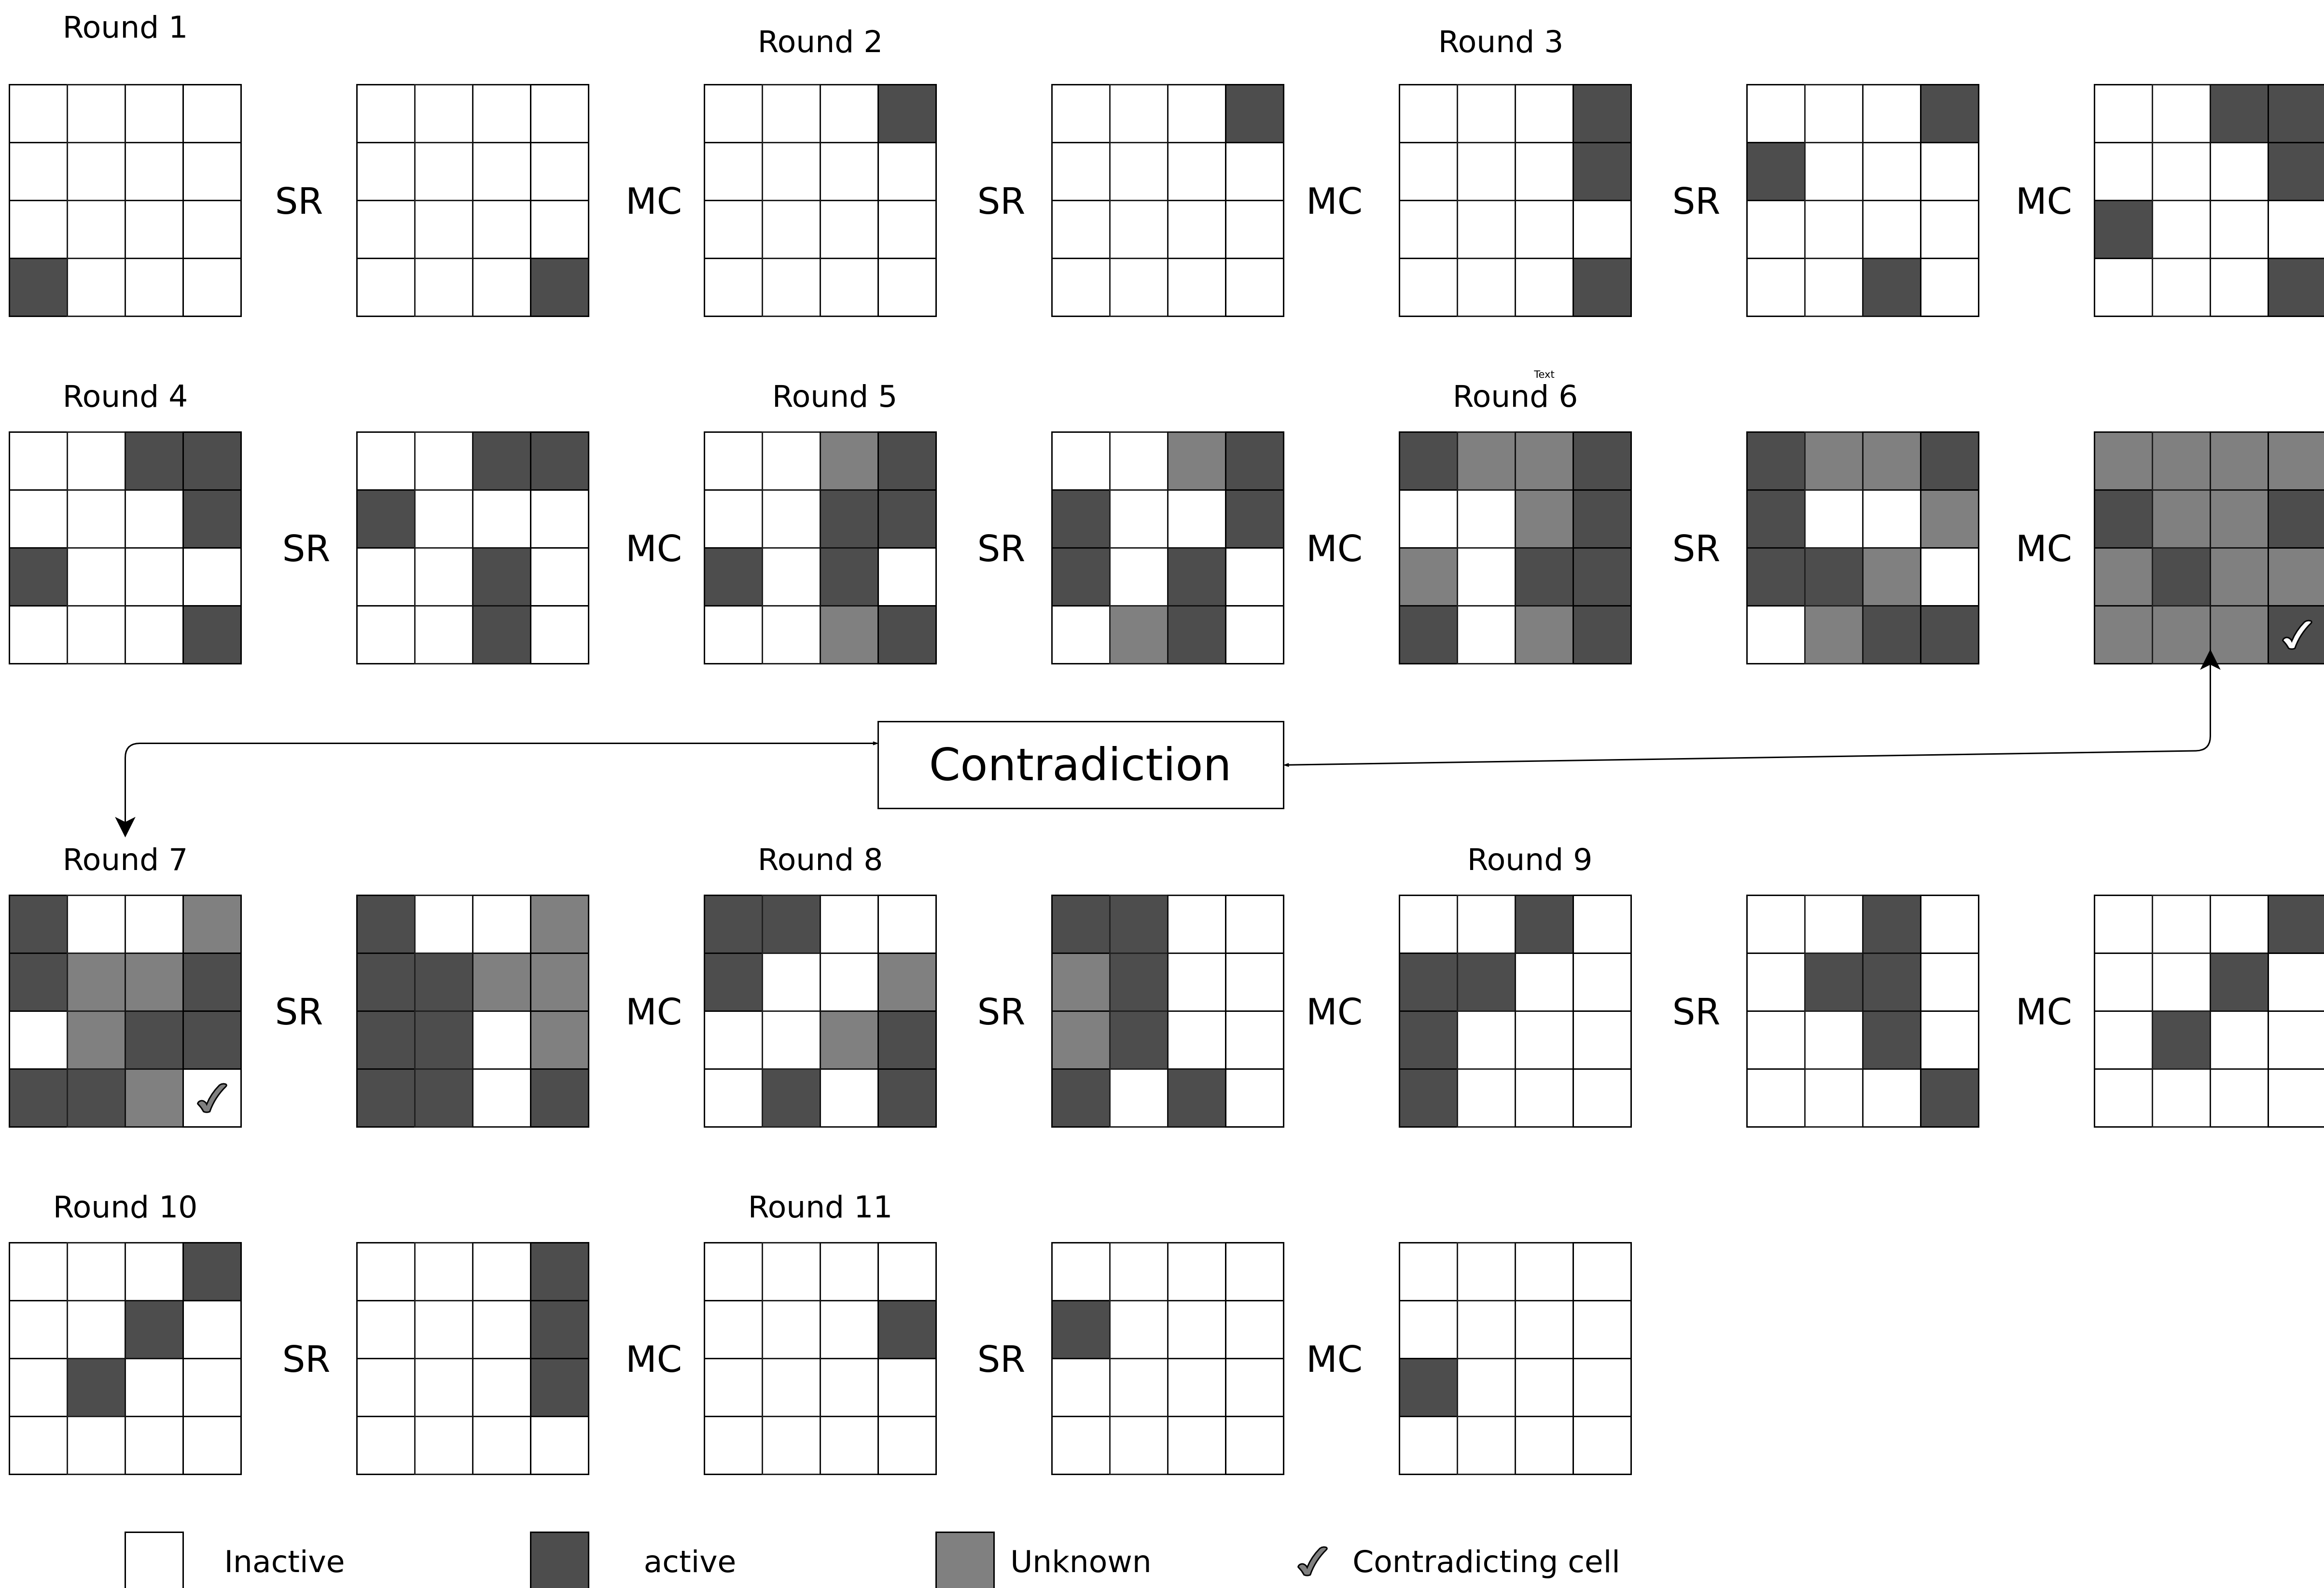
\includegraphics[width=10cm]{fig3.png}
\end{figure}
Now we will find the maximum number of rounds, so that we get any non-trivial properties.For
this we do or follow an Experiment.Initially we set only one active cell to the state. And encrypt
until we all cells become Unknown and in the process, we use different values of constant cells
and tweakey.\\
\tab$\quad\quad$As a result, we found that an active cell in any of the third row will yield two cells satisfying the
property after seven rounds.\\ \\
\tab$\quad\quad$Property is extended to higher order by changing active cells in the backward direction.
Ex:- property can be extended by 4 round in backwards by activating 12 cells and in the end we
get 10 round integral distinguisher can be constructed

\begin{figure}[H]
	\centering
	\caption{16-round key recovery with impossible differential attack for SKINNY-64 with 64-bit tweakey and SKINNY-128 with 128-bit tweakey.}
	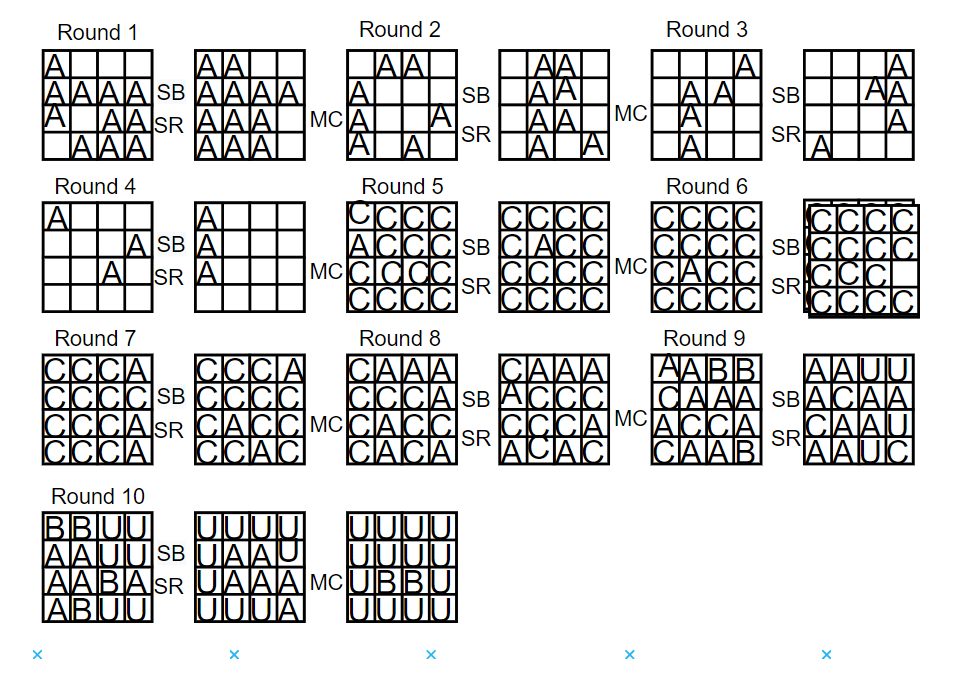
\includegraphics[width=10cm]{fig5.png}
\end{figure}
We take about algebraic degree of the 4-bit sbox and 8 bit sbox, Then in 4 bit sbox algebraic
degree is 3 while 8 bit sbox is 6.Thus the integral property of Skinny 128 can be longer than
Skinny.Now we see how these three properties help us to recover 4 rounds.After the 10-round
integral distinguisher we go 4 rounds in forward.So that we will attack on backward and reach
10-round.\\ \\
Process(Follow the figure):-\\
\textbf{1)} First we prepares $2^{12c}$ plaintext for integral distinguisher.After that we compute inverse
MixColumns for each ciphertext.then we change 4-cell values for proceed backward
computation.Now we have 8 active cell. Now our remaining text size is $2^{8c}$.\\
\textbf{2)} Actually we are going backward, so we know all the ciphertext, in 13 rounds we again invers
SubCells and MixColumns.we can see in the figure we again change 4 cells to our properties. In
this step guess data and compute, before this we have $2^8c$ data. For this we perform \\$2^{8c}$.
$2^{4c}$ = $2^{12c}$. Now our remaining text size is $2^{5c}$.\\
\textbf{3)} Given $2^{5c}$ data,we again compute inverse MixColumns in round-12 for each ciphertext.then
we change 2-cell values for proceed backward computation. For this we need $2^{6c}$ guesses.\\
which requires $2^{11c}$ computation.\\
\textbf{4)} Given 2$^{2c}$ data,we again compute inverse MixColumns in round-11 for each ciphertext.then
we change 1-cell values to proceed backward computation.\\
\textbf{5)} Computed results are tested if the Balanced (B) property is satisfied. The guessed
10-cell key candidates are reduced by a factor of $2^{-3c}$.\\
\begin{figure}[H]
	\centering
	\caption{10 round integral distinguisher.}
	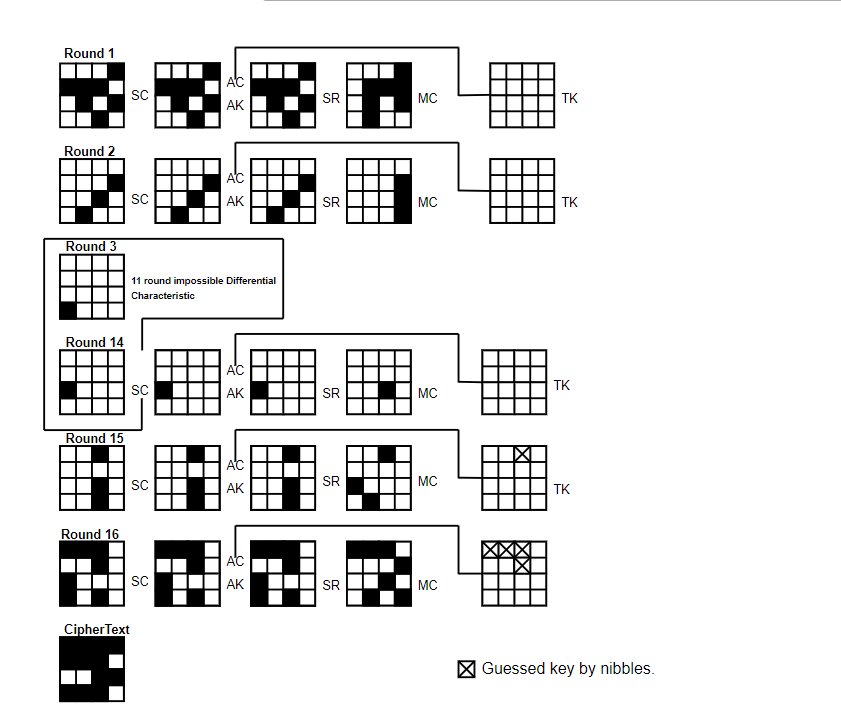
\includegraphics[width=10cm]{fig4.png}
\end{figure}
So memory, data, computation required in this attack are following
memory $2^{12c}$, data $2^{12c}$, computation $2^{12c}$)\\
Where c is the size of the cell.
\subsection{Impossible Differential Attacks}
\tab In this attack, attackers find two internal state differences, where both states never propagate to
each other.\\
\tab$\quad\quad$like if we have two states $\backslash$del and $\backslash$del', the $\backslash$del is never propagated to $\backslash$del' other.
After that the attacker finds many plain text and ciphertext and tweakey values, those are
leading to \\( $\backslash$del, $\backslash$del'). If any tweakey value is wrong, then we will reduce from tweakey space.
\tab$\quad\quad$Basically in this analysis ,with the help of miss-in-the-middle We find impossible differential
characteristics technique , for these we took 16 input truncated differentials and 16 output
truncated differentials with single active cells propagated with encrypt and decrypt function.
and Until no cell can be active or inactive with probability one, then we pick up the pair
contradicting each other in the middle.\\
And in the end we get the longest impossible differential characteristics to reach 11 rounds with
16 such characteristics in total.\\
(0, 0, 0, 0, 0, 0, 0, 0, 0, 0, 0, 0, $\triangle$, 0, 0, 0) 12R $\Rightarrow$ cut (0, 0, 0, 0, 0, 0, 0, 0, $\triangle$0, 0, 0, 0, 0, 0, 0, 0).\\
\tab$\quad\quad$And we can also add several round before and after the 11 round impossible differential
characteristics, and number of round depend on key size, if block size and key size are same
then after add two round before and three round after, we get plaintext differences
\\(0, 0, 0, *, *, *, *, 0, 0, *, 0, *, 0, 0, *, 0) and the ciphertext difference becomes and the
ciphertext difference becomes (*, *, *, *, *, *, *, 0, 0, 0, *, *, *, *, *, 0) where * is non-zero
different.\\
\begin{figure}[H]
	\centering
	\caption{16 round key recovery with Integral Attack for 64-bit SKINNY cipher.}
	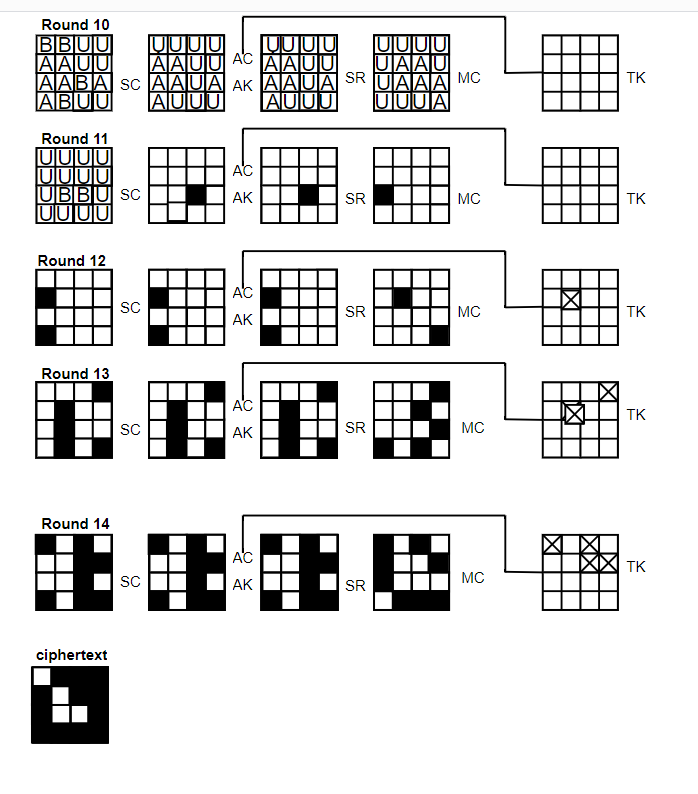
\includegraphics[width=10cm]{fig6.png}
\end{figure}
In this Cipher AddroundTweakey, shiftrow and Mixcolumn are effect on each other between
different states.\\
\tab$\quad\quad$And the number of tweakey cells involved is 3 in the first tree round while 5 in the last tree
round. So 8 cells in total.
\subsection{Meet-In-The-Middle Attacks}
\tab This attack has been applied to block ciphers. Basically it works on SPN structure. We only see
some definition or process. Not a proof.
According to this Number of attacked rounds can be calculated by considering the maximum
length of these three features.\\
\tab$\quad\quad$\textbf{Partial-Matching} If Number of rounds reaches full diffusion rounds in both
directions(backward and forward). In SKINNY full diffusion is achieved after 6 rounds forward
and backward.
then Partial-Matching on work at most 10 ((6-1)+(6-1)) rounds.\\
\tab$\quad\quad$\textbf{Initial structure} This structure can also be bounded by a smaller number of full diffusion
rounds in both directions(backward and forward).
and it works up to 7 (6+2-1) rounds for SKINNY.\\
\tab$\quad\quad$\textbf{Splice-and-cut} It is also the same as Initial structure, and it may extend the Number of
rounds up to the same number of full diffusion rounds minus one (means 6-1=5). And it the end,
we get a total 10+7+5=22 round from Meet-In-The-Middle Attacks.\\
So we can say 32+ rounds of SKINNY can provide a valuable security margin.

\section{Implementations}
\subsection{Round Based Implementation}
\tab In particular, SKINNY-64-128 offers the smallest area footprint compared to other
lightweight ciphers providing the same security level. Note, that even SIMON-64-128
implemented in a round-based fashion cannot compete with our design in terms of area
although it has a smaller critical path, hence can be operated at higher frequencies and
provides better throughput. However, comparing the throughput at a frequency of 100KHz,
SKINNY provides better results since the number of rounds is substantially lower than for
SIMON.

\begin{table}[hbt]
	\centering
	\begin{tabular}{lllllll}
		\hline
		\multirow{3}{*}{} &
		\multirow{2}{*}{Area} &
		\multirow{2}{*}{Delay} &
		\multirow{2}{*}{\begin{tabular}[c]{@{}l@{}}Clock\\ Cycles\end{tabular}} &
		\multicolumn{2}{l}{Throughput} &
		\multirow{3}{*}{Ref.} \\ \cline{5-6}
		&      &      &    & @100KHz & @maximum &     \\ \cline{2-6}
		& GE   & ns   & \# & KBit/s  & MBit/s   &     \\ \hline
		SKINNY-64-64   & 1223 & 1.77 & 32 & 200.00  & 1130.00  & New \\ 
		SKINNY-64-128  & 1696 & 1.87 & 36 & 177.78  & 951.11   & New \\ 
		SKINNY-64-192  & 2183 & 2.02 & 40 & 160.00  & 792.00   & New \\ \hline
		SKINNY-128-128 & 2391 & 2.89 & 40 & 320.00  & 1107.20  & New \\ 
		SKINNY-128-256 & 3312 & 2.89 & 48 & 266.67  & 922.67   & New \\ 
		SKINNY-128-384 & 4268 & 2.89 & 56 & 228.57  & 790.86   & New \\ \hline
	\end{tabular}
\caption{Round based implementations of SKINNY-64 and SKINNY-128}
\end{table}

\subsection{Serial Implementation}
\tab Serial implementations have the smallest area footprint for hardware implementations
by updating only a small number of bits per clock cycle. However, the throughput and
performance of such implementations is decreased significantly. Often, only a single instance
of an Sbox is implemented and re-used to update the internal state of the round function
in a serial fashion. Depending on the size of the Sbox, we call these implementations
nibble-serial (4-bit Sbox) or byte-serial (8-bit Sbox), respectively. Besides, we provide bit-serial implementations for SKINNY-64 and SKINNY-128
which update only a single bit of the round state per clock cycle. These implementations
benefit from the iterative structure of both 4- and 8-bit Sboxes of SKINNY allowing to
compute them bit by bit in 4 respectively 8 clock cycles.
\subsection{FPGA Implementations}
\tab A brief summary of implementation results for high-performance architectures on
FPGAs for both, SKINNY-64 and SKINNY-128.
Most reference implementations found in the
literature either do not target fully pipelined and unrolled implementations or just provide
results for older FPGA technologies using 4-input LUTs instead of 6-input LUTs found
in modern devices. Still, we would like to highlight the performance figures of all of our
SKINNY implementations for FPGAs allowing to implement high-performance architectures
at a minimum of resource consumption.
\subsection{Micro-Controller Implementations}
\tab In this section, we describe the main performance figures when implementing SKINNY on
micro-controllers. We omit details of the implementation and mainly describe the results
of the implementation.\\
\tab$\quad\quad$A lot of different trade-offs can be made, which is a real strength of SKINNY, since
different applications may have very different requirements and total costs would be
computed very differently, sometimes justifying sacrifices which would be unacceptable in
most cases. In Table 5, we provide several of those trade-offs, each optimizing for another
of the three criteria mentioned above.\\
\begin{table}[hbt]
	\centering
	\begin{tabular}{lllllll}
		\hline
		Cycles per byte & 222 & 257 & 258 & 288 & 297 & 328 \\
		RAM             & 576 & 287 & 576 & 287 & 31  & 31  \\
		ROM             & 676 & 616 & 492 & 436 & 774 & 594 \\ \hline
	\end{tabular}
\caption{Implementation figures for SKINNY-128-128 on an ATmega644}
\end{table}

\section{Conclusion}
\tab Going through the family of SKINNY ciphers we have compared SKINNY and its Low-Latency Variant MANTIS, we have gone throught different aspect of this cipher. Comparision with the algorithm, security, implementations, attacks with the use of different modals and tables. Providing different implementation and corresponding to that impementation, providing corresponding proof for claming that thing.\\
\tab$\quad\quad$ We presented a  tweakable block cipher family SKINNY. Then we presented MANTIS, a dedicated variant of SKINNY for low-latency implementations, that constitutes a very efficient solution to the problem of designing a tweakable block cipher for memory encryption. We discussed Rationale of SKINNY, Estimating Area and Performances, General Design and Components Rationale, Security analysis,  Differential/Linear Cryptanalysis, Meet-in-the-Middle Attacks, Impossible Differential Attacks, ASIC implementations, round-based implementations, Unrolled Implementation, Serial Implementation etc. We like to thank Daniel Otto for providing us with performance figures for SKINNY on micro-controllers.

\section{Brownie Points}
\subsection{Integral Attacks}
\tab This is nominated becuse of some points being spacial and this was the attack also. Round are being added so it makes it interesting. There are 11 round which are impossible differential characteristic.
%%%% 8. BILBIOGRAPHY %%%%
\bibliographystyle{alpha}
\bibliography{abbrev3,crypto,biblio}
1. Guo, J., Peyrin, T., Poschmann, A., Robshaw, M.J.B.: The LED block cipher. [37] 326–341\\
2. Nikova, S., Rijmen, V., Schläffer, M.: Secure Hardware Implementation of Nonlinear Functions
in the Presence of Glitches. J. Cryptology 24(2) (2011) 292–321\\
3. Piret, G., Roche, T., Carlet, C.: PICARO - a block cipher allowing efficient higher-order
side-channel resistance. In Bao, F., Samarati, P., Zhou, J., eds.: ACNS 12. Volume 7341 of
LNCS., Springer, Heidelberg (June 2012) 311–328\\
4. Banik, S., Bogdanov, A., Isobe, T., Shibutani, K., Hiwatari, H., Akishita, T., Regazzoni, F.:
Midori: A Block Cipher for Low Energy. In: Advances in Cryptology - ASIACRYPT 2015 -
Part II. Volume 9453 of Lecture Notes in Computer Science., Springer (2015) 411–436\\
5. National Institute of Standards and Technology:
Recommendation for Key Man-
agement – NIST SP-800-57 Part 3 Revision 1. http://nvlpubs.nist.gov/nistpubs/
SpecialPublications/NIST.SP.800-57Pt3r1.pdf\\
6. Wingers, L.: Software for SUPERCOP Benchmarking of SIMON and SPECK. https:
//github.com/lrwinge/simon\_speck\_supercop (2015)\\
7. Daemen, J., Peeters, M., Assche, G.V., Rijmen, V.: Nessie Proposal: the Block Cipher
Noekeon. Nessie submission (2000) http://gro.noekeon.org/.\\
8. Sun, S., Hu, L., Song, L., Xie, Y., Wang, P.: Automatic security evaluation of block ciphers
with s-bp structures against related-key differential attacks. In: Inscrypt 2013. (2014) 39–51
%%%% NOTES
% - Download abbrev3.bib and crypto.bib from https://cryptobib.di.ens.fr/
% - Use bilbio.bib for additional references not in the cryptobib database.
%   If possible, take them from DBLP.

\end{document}
